%%%%
\newpage
\section{Fluorescência de Raios X}

Para quantificar a composição elementar (número atômico $ 10 < Z < 82$) das 
amostras foi utilizada a técnica não-destrutiva de Fluorescência de Raios X 
(XRF), um método analítico quali-quantitativo, multielementar, 
que mede os raios X característicos emitidos pelos átomos da amostra, 
depois de também serem excitados por raios X. Permite análise simultânea dos 
elementos químicos e não exige pré-tratamento dos alvos.

Há basicamente 3 etapas envolvida na técnica de medida de raios X 
característicos: excitação da amostra, emissão de raios X pelos átomos da amostra
e detecção. A excitação pode ocorrer por feixe de raios X (ou raios gamas) 
produzido em fontes radioativas, por partículas aceleradas 
(elétrons, prótons, alfas etc) ou 
por tubos geradores de raios X quando submetidos a diferença de potencial
\citep{jenkins1988}. 

No caso da XRF, a excitação ocorre por um feixe de raios X incidente, que  
expulsa os elétrons das camadas mais internas do átomo (K,L e M) 
produzindo vacâncias. Para tal, a energia do feixe incidente deve ser maior 
que a energia de ligação dos elétrons nessas camadas. Um átomo com vacância é 
instável e rapidamente elétrons das camadas mais externas preenchem as vacâncias,
liberando fotóns e estabilizando o átomo, sendo a energia destes fótons 
correspondentes às energias de transição entre camadas do átomos, 
característica de cada elemento químico. O processo de excitação do átomo 
é ilustrado classicamente na figura \ref{fig:shimadzu_atomo}.

\begin{figure}[H]
  \centering
  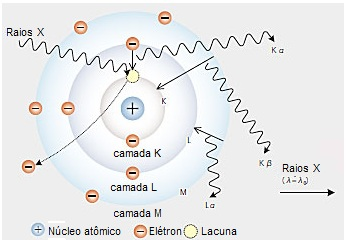
\includegraphics[width=0.5\textwidth]{../inputs/images/shimadzu_atomo.jpg}
  \caption{Ilustração clássica do fenômeno de fluorescência de raios X no átomo. 
           Figura acompanha o manual da Shimadzu da série de equipamentos
           EDX 700 \label{fig:shimadzu_atomo}}
\end{figure}

As transições dos elétrons entre os níveis quânticos K, L e M encontram-se 
tipicamente na faixa dos raios X, tendendo a ultravioleta (UV) e luz visível,
conforme ocorram em transições atômicas de menor energia no átomo.

Transições da camada L para K são do tipo $K_{\alpha}$, de M para K 
são $K_{\beta}$ e de M para L são $L_{\alpha}$ ou $L_{\beta}$. 
As camadas L e M possuem ainda subníveis de energia, o que resulta em diversas
combinações de transições, sendo algumas delas proibidas, e outras 
com diferenças de energia indistinguíveis para os detectores utilizados 
neste método analítico (XRF-ED).

A notação desenvolvida por Siegbahn \citep{jenkins1991}, 
com as principais transições possíveis sintetizada na figura \ref{fig:siegbahn},
permite identificarmos melhor os subníveis de origen e destino, por exemplo, 
a transição de $M_{IV}$ para $L_{III}$ é uma transição do tipo $L_{\beta_1}$,  . 

\begin{figure}[H]
  \centering 
  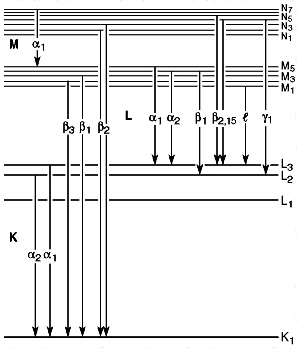
\includegraphics[width=0.5\textwidth]{../inputs/images/Siegbahn.jpg}
  \caption{Transições de elétrons entre os subníveis das camadas K, L e M. 
           Figura extraída de \citet{jenkins1991} \label{fig:siegbahn}}
\end{figure}

Na prática, dependendo do modo de detecção dos raios-X, agrupa-se transições 
dos subníveis e trabalha-se com as denominações de linhas K e L apenas. As linha
$K_{\alpha}$ são as mais intensas, oferecendo melhor limite de detecção
para um elemento. Mas elas também são as mais energéticas, podendo ultrapassar a
faixa de sensibilidade do detector empregado. Nestes casos as linhas L passam a 
ser analisadas. No modelo de XRF usado nesta pesquisa, analisou-se as linhas K, 
desde o sódio (Na) até molibdênio (Mo), e as linha L, do molibdênio (Mo)
até o chumbo (Pb).  
 
%%%%
\subsection{Tipos de XRF}

Há essencialmente dois tipos principais de equipamentos de XRF que se 
diferenciam pelo modo como os raios X são detectados: fluorescência de raios 
X dispersivo em comprimento de onda (XRF-WD) e fluorescência de raios X 
dispersivo em energia (XRF-ED).

Na XRF-WD os raios X da amostra sofrem difração em um cristal, quantificando-se
os elementos químicos pela contagem de fótons nos ângulo de difração $\theta$, 
característicos dos elementos, segundo a lei de Bragg:

\begin{equation}
	\label{eq:bragg}
	2d sen(\theta) = n \lambda
\end{equation}

Onde, $d$ a distância entre planos do cristal, $\theta$ o ângulo de incidência 
em relação ao plano considerado, $\lambda$ o comprimento de onda 
(e, portanto, a energia) da radiação incidente e $n$ um inteiro.
Esse tipo de equipamento permite uma grande resolução dos comprimentos de onda 
(energia) característicos dos elementos, facilitando detectá-los e, geralmente, 
com bom limite de detecção (LD).
Entretanto apresentam diversos problemas práticos quando empregados em filtros 
de aerossol atmosférico. Em função disso há uma preferência pelos sistemas 
dispersivos em energia nesse campo de análise. 

A XRF-ED usa detectores de semicondutores capazes de discriminar energias 
próximas com alta resolução temporal, viabilizando a detecção simultânea dos 
elementos químicos através da amplitude do pulso eletrônico produzido no 
detector, proporcional à energia do fóton incidente. O sistema eletrônico do 
equipamento faz a conversão analógica-digital da intensidade do pulso, 
acumulando a contagem por energia em um multicanal. O detector mais empregado é 
o de silício ativado com lítio Si(Li). 

Neste sistema o LD das análises é particularmente limitado pelos raios-X de 
excitação que sofrem reflexão na amostra e também chegam ao detector. 
Formam assim uma contagem de fundo (\textit{background}) que concorre com 
aquela proveniente dos picos característicos. 
Fluorescência de raios X polarizada (XRF-EDP) e fluorescência de raios X por 
reflexão total (XRF-T) são dois sistemas que têm sido empregados 
para reduzir o \textit{background} e melhorar significativamente o LD.

Na XRF-EDP excita-se a amostra com raios X polarizados e se ajusta o ângulo 
de detecção a 90 $\degree$ deste feixe \cite{dzubay1974}. Nesta direção a 
reflexão do feixe incidente polarizado é pequena, obtendo-se grande redução 
na intensidade do fundo e, consequentemente, no LD, tipicamente fator 2 a 10
dependendo do elemento e das condições de irradiação comparadas 
(Meel K. V., 2009).

%Meel, 2009
%Meel, Katleen Van, 2009. Application of high-energy polarized-beam energy-dispersive X-ray fluorescence for industrial and environmental purposes. Doctoral Thesis, Universiteit Antwerpen, Faculteit Wetenschappen, Departement Chemie. Orientador: René Van Grieken; p. 154.  

A XRF-T emprega a propriedade da radiação eletromagnética incidente abaixo do
ângulo crítico sobre uma superfície. Incidindo-se um feixe que resvale a amostra
com um ângulo bem pequeno, este excitará uma fina camada da superfície, 
penetrando muito pouco no suporte. Desta forma um detector posicionado 
perpendicularmente à superfície receberá muitos fótons característicos gerados 
pela amostra e pouco fundo refletido no suporte, melhorando o LD
\citep{yoneda1971} e \citep{aiginger1974}.

%%%%
\subsection{Características da XRF-ED utilizada}

Neste trabalho foi utilizado uma XRF-ED da marca Shimadzu modelo EDX 720HS, 
apresentado na figura \ref{fig:xrfed_iag},
pertencente ao Laboratório de Poluição atmosférica Experimental (LAPAE) 
da Faculade de Medicina da USP e instalado no LAPAt. 

\begin{figure}[H]
  \centering
  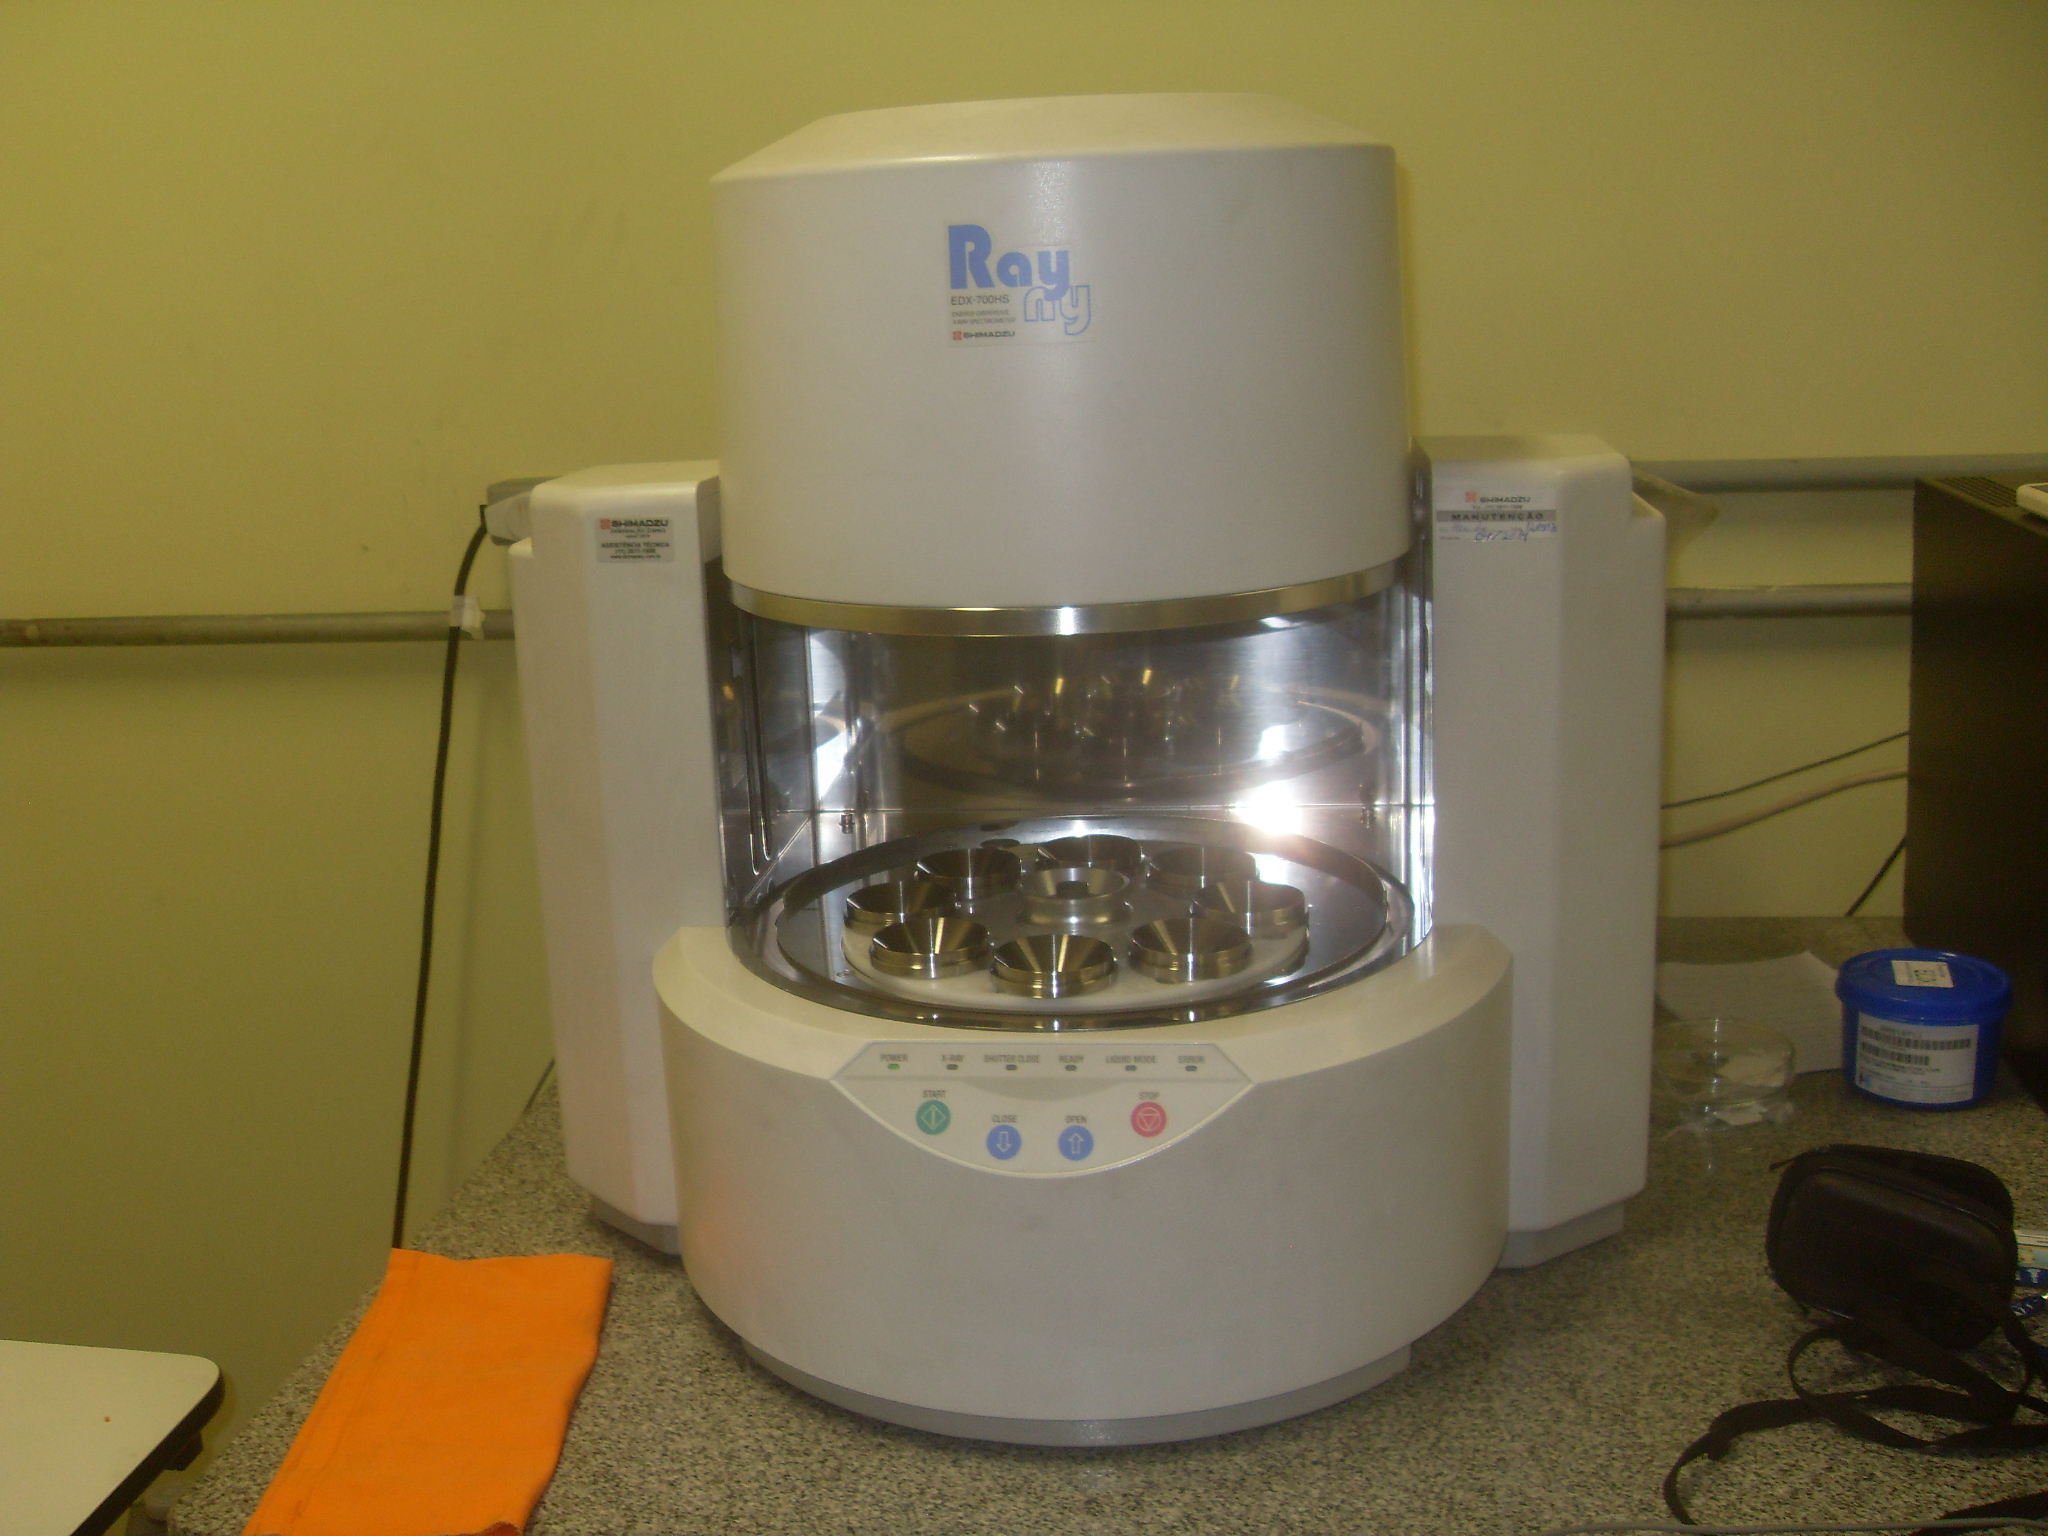
\includegraphics[width=0.5\textwidth]{../inputs/images/xrf-ed-IAG-USP.jpg}
  \caption{ED-XRF Shimadzu modelo EDX 720HS - LAPAt \label{fig:xrfed_iag}}
\end{figure}

Um tubo de ródio (Rh) submetido a uma diferença de potencial 
de 50 kV foi utilizado para geração do feixe de raios X.
O detector de silício ativado com lítio Si(Li) possui sensibilidade
para medida de fótons com energia entre 1 e 20 keV acoplado a um sistema 
eletrônico com multicanal de 2048 canais capaz de quantificar simultaneamente 
os elementos desde o Na até o Pb. Para remoção da radiação da linha L do feixe 
de raios X do tubo de ródio, de energia próxima de 2,6 keV, um filtro de 
alumínio foi posto entre o feixe e a amostra, melhorando o limite de detecção 
dos elementos com energia igual ou menor que 2,6 keV. O diâmetro do feixe de 
raios X é definido por um colimador de 10 mm, garantindo a irradiação de uma 
área representativa e homogênea da amostra. 

O tempo vivo de irradiação de cada amostra foi $\pm$ 960 minutos, ajustando-se 
a corrente para manter o tempo morto em 20\%. Desejava-se desta forma fixar a 
taxa de contagem, obtendo-se ao final o mesmo número total de fótons contados 
em cada espectro. Esse mecanismo permite melhorar o LD dos elementos presentes 
em amostras menos carregadas. Isso nem sempre foi possível já que a corrente 
máxima no tubo gerador de raios X era de 1000 $\mu A$. 

A figura \ref{fig:xrfed_software} foi extraída do software que acompanha o 
equipamento da Shimadzu e permite verificar em tempo real características
da análise como a voltagem e corrente no tubo, se há filtro e qual, 
informação sobre o vácuo na câmera, dentre outros dados que ajudam a conferir se 
a análise está sendo realizada como planejado. 

\begin{figure}[H]
  \centering
  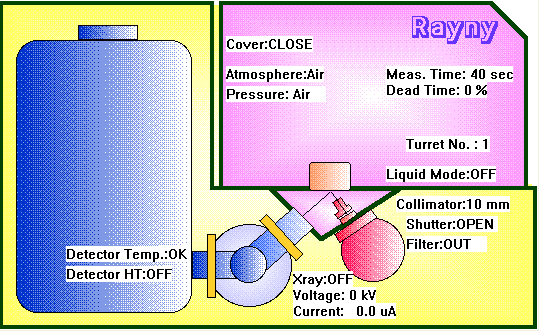
\includegraphics[scale=0.4]{../inputs/images/edx_iag_monitor.png}
  \caption{Software da ED-XRF Shimadzu 720HS, tela de verificação 
           do estado do equipamento. \label{fig:xrfed_software}}
\end{figure}

O EDX 720HS permite análise automática de amostras encaixadas em carrosséis 
de 8 ou 16 posições. O LAPAt contava então apenas com o carrossel de 16 
posições. Foi necessário adquirir um com 8 posições, cujos receptáculos admitiam
o maior diâmetro dos filtros de PTFE, que não podem ser cortados e remontados 
como os de policarbonatos (figura \ref{fig:carrossel8}).

\begin{figure}[H]
  \centering
  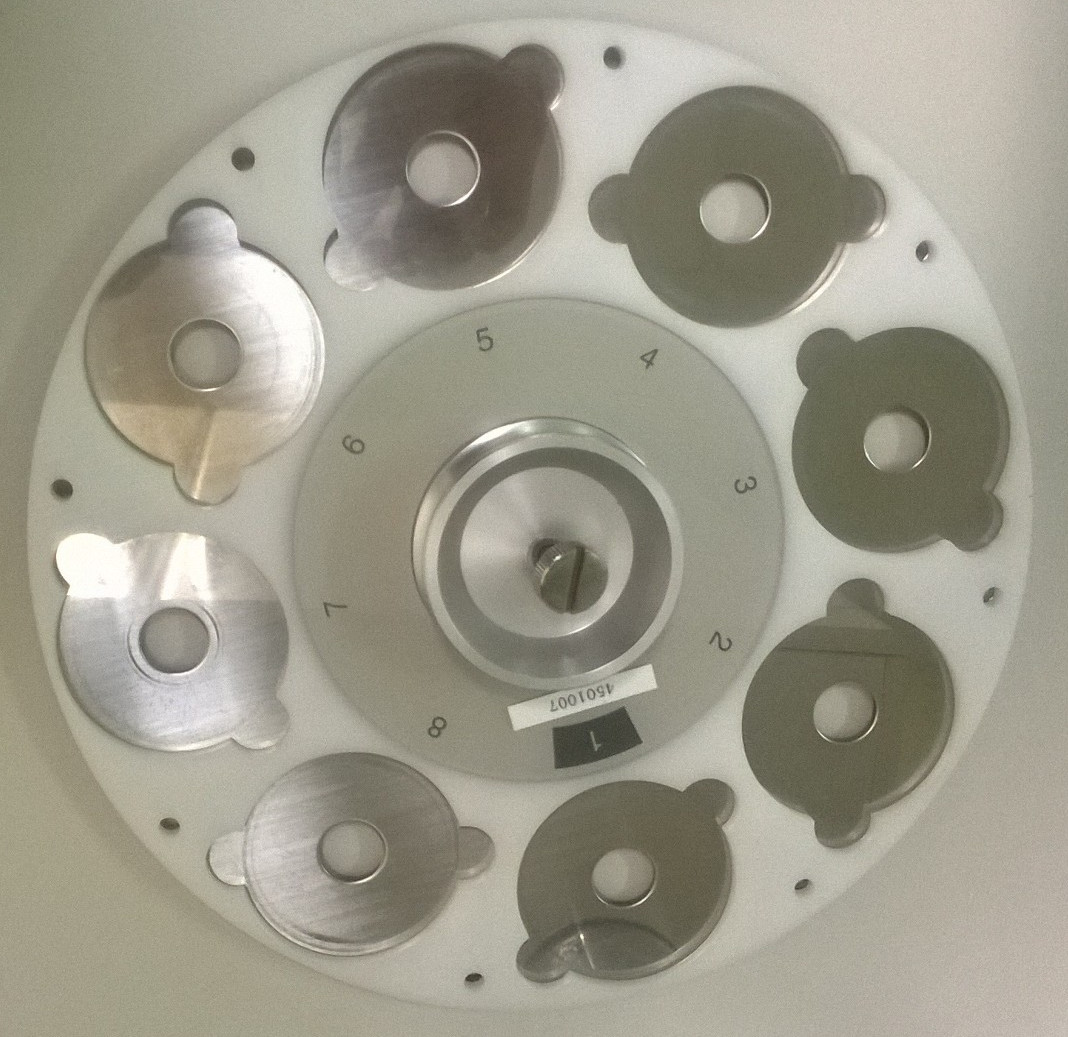
\includegraphics[width=0.5\textwidth]{../inputs/images/carrossel8.jpg}
  \caption{Carrossel de 8 posições adquirido para XRF-ED Shimadzu 720HS. 
           \label{fig:carrossel8}}
\end{figure}

Para eliminar as ondulações típicas que ocorrem nos filtros de PTFE, 
projetou-se um suporte de aço inox que comprimia sua moldura, mantendo plana 
a superfície a ser analisada. Ao mesmo tempo, o peso deste suporte impedia que 
o filtro "voasse" quando era feito ou quebrado o vácuo na câmera 
(figura \ref{fig:suporte8}).

\begin{figure}[H]
  \centering
  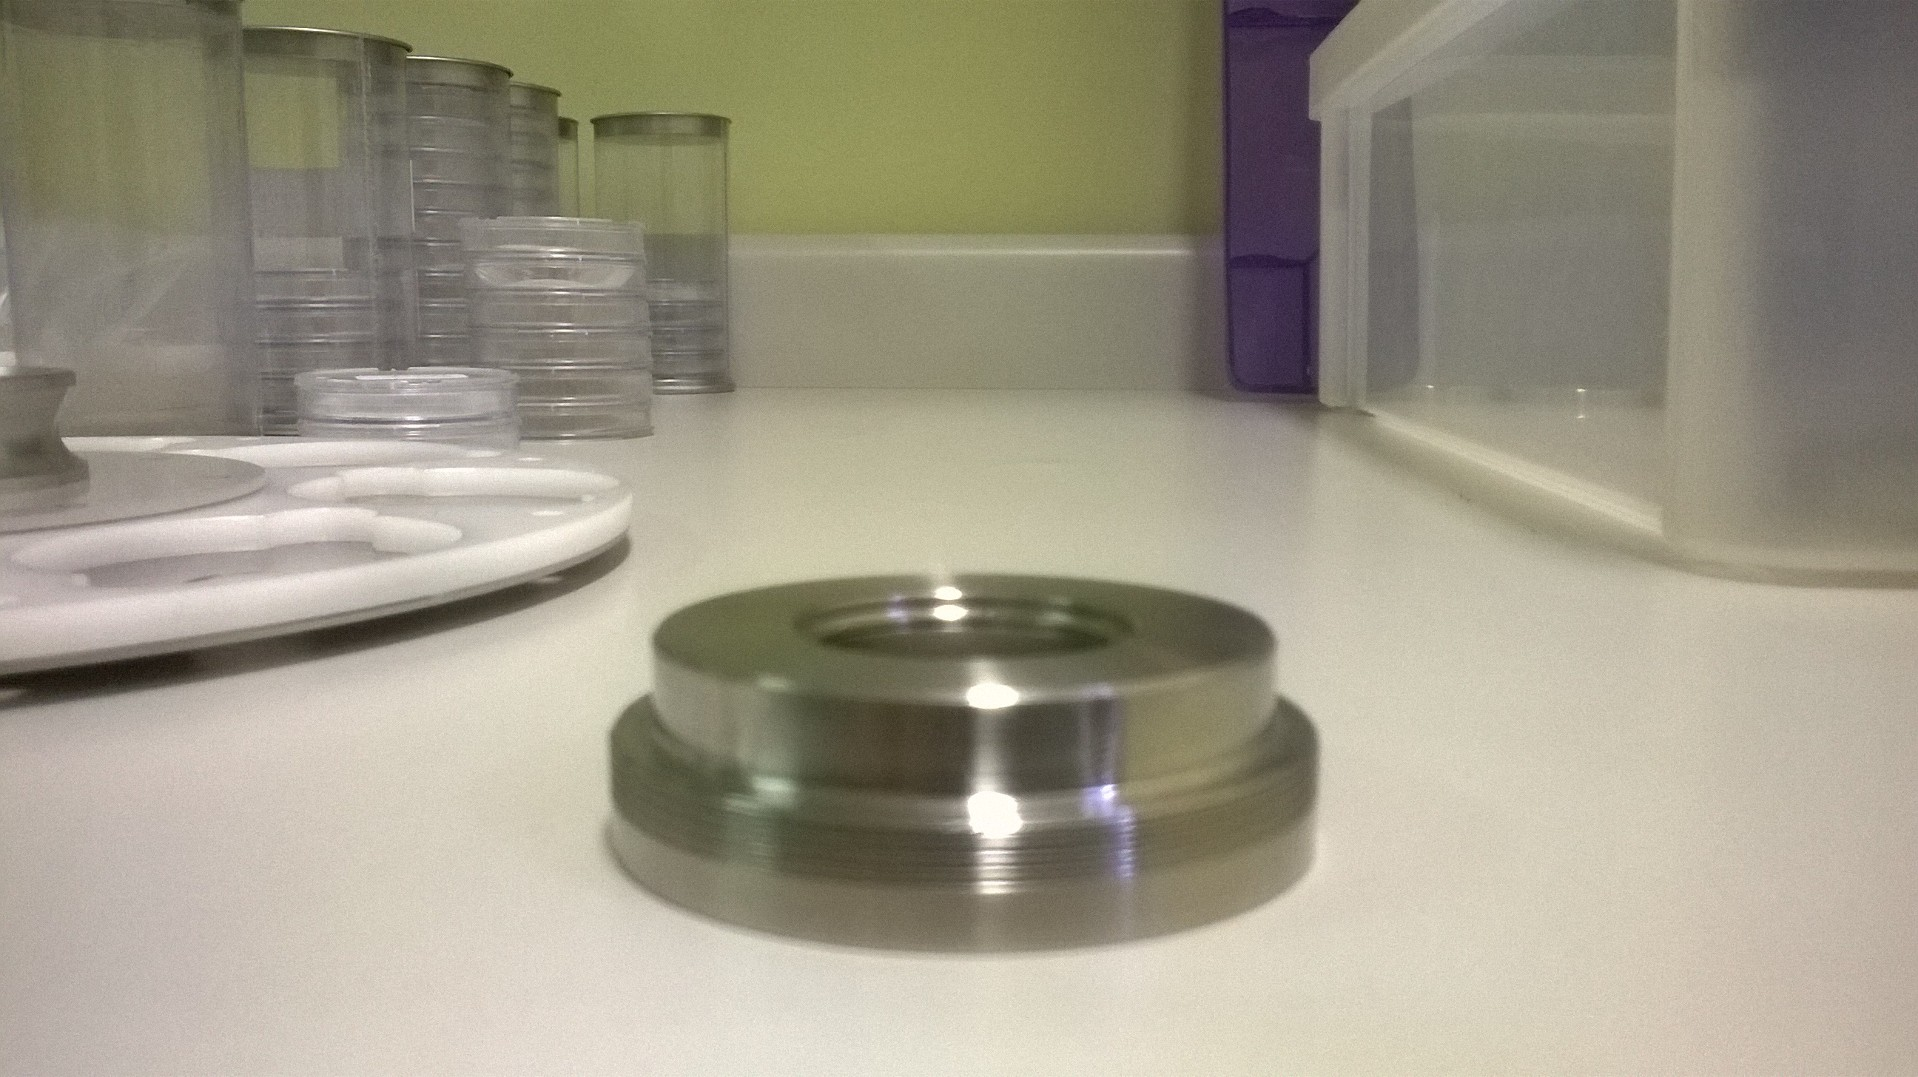
\includegraphics[width=0.5\textwidth]{../inputs/images/suporte8.jpg}
  \caption{Suporte para filtros de PTFE, projetado no LAPAt para carrossel de 
           8 posições e produzido pela oficina da FAP no 
           Instituto de Física da USP. \label{fig:suporte8}}
\end{figure}

%%%%
\subsection{Calibração do ED-XRF}

A massa por unidade de área, depositada sobre os filtros tipicamente usados em 
pesquisas de aerosol atmosférico, permite tratá-los como amostras finas,
ou seja, o efeito de matriz, interações dos raios X característicos com os 
elementos da amostras causando absorção ou reforço do número de fótons de 
raios X característicos, são pequenos diante da precisão do método,
podendo-se desconsiderá-lo. Nesta aproximação, pode-se relacionar de modo 
simples o número de fótons contados sob o pico característico de um elemento, 
presente no espectro obtido, com a sua massa na amostra irradiada:

\begin{equation}
  \label{eq:contagem}
  N(Z) = R(Z) \cdot I \cdot \Delta t  \cdot \frac{m(Z)}{A}
\end{equation}

Onde R(Z) é chamado de fator de resposta, I é a corrente de excitação do tubo 
de raios X, determinando, portanto, o fluxo de raios X que chegam à amostra, 
$\Delta t$ é o tempo vivo de irradiação e m(Z)/A é a densidade 
(massa por unidade de área) dos elementos Z presentas na amostra. 
Nota-se pressupõe-se distribuição uniforme da massa na superfície do filtro.

O termo R(Z) depende da seção de choque de cada elemento com o feixe de 
raios X incidente (incluindo modificações por eventuais filtros moduladores 
de suas características), da curva de eficiência do detector de raios X, 
da eficiência de operação do tubo de raios X e da geometria do sistema, 
incluindo os diâmetros de colimadores selecionados. Mantendo estes parâmetros 
fixos e irradiando-se alvos padrões com densidades (d(Z) = m(Z)/A) 
conhecidas, pode-se calcular R(Z):

\begin{equation}
  \label{eq:fator_de_resposta}
  R(Z) = \frac{N(Z)}{d(Z) \cdot I \Delta t}
\end{equation}

Considerando que a incerteza da corrente e do tempo vivo são desprezíveis 
perto da incerteza da densidade e da contagem, a incerteza no fator de resposta
pode ser calculada por propagação de erro destas variáveis:

\begin{equation}
  \label{eq:erro_fator_de_resposta}
  \sigma_{R(Z)}^2 = {R(Z)}^2 \cdot \left( \left(\frac{\sigma_{N(Z)}}{N(Z)}\right)^2 + 
                                      \left(\frac{\sigma_{d(Z)}}{d(Z)}\right)^2 
                                   \right)
\end{equation}

Dados ambientais são reportados em medidas de concentração ($\mu g/m^3$),
razão da massa m(Z) pelo volume amostrado. Conhecendo-se o fator de resposta 
R(Z) pode-se calcular a massa m(Z) depositada na amostra, usando a equação 
\ref{eq:contagem}, tomando como valor da área A com deposição de aerossol
no filtro:

\begin{equation}
  \label{eq:xrfedmassa}
  m(Z) = \frac{N(Z) \cdot A}{ R(Z) \cdot I \cdot \Delta t}
\end{equation}

Empregando-se novamente a expressão da propagação de erro para variáveis 
independentes, a incerteza na massa será:

\begin{equation}
  \label{eq:erro_massa}
  \sigma_{m(Z)}^2 = {m(Z)}^2 \left( \left(\frac{\sigma_{N(Z)}}{N(Z)}\right)^2 + 
                                  \left(\frac{\sigma_A}{A}\right)^2 + 
                                  \left(\frac{\sigma_{R(Z)}}{R(Z)}\right)^2 
                             \right)
\end{equation}


Vê-se, entretanto, que para cada espécie química de interesse, seria necessário
ao menos um alvo de calibração para calcular seu R(Z). Alvos padrões finos, 
com densidade elementar conhecida, podem ser comprados ou produzidos, dependendo
da precisão desejada. Neste projeto foram adquiridos alvos padrões da 
Micromatter, com incerteza nominal de 5\%. Mas esta empresa não produz alvos 
com proporção estequiométrica quantificada para todas espécies químicas.
Assim, trouxemos para a XRF-ED o conceito proposto por \citep{tabacniks2000}
para o sistema PIXE (Particle Induced X-Ray Emission) que permite obter uma 
calibração abrangendo elementos de número atômico no intervalo 10 < Z < 83. 
 
Empregou-se, ainda, uma metodologia estatística robusta para estimativa das 
incertezas para a calibração usando MQM. Essa preocupação em definir 
adequadamente as incertezas deve-se, particularmente, ao fato de que elas 
ponderam o peso das variáveis na modelagem por PMF.

Como exemplo para conhecer o forma da curva de calibração, o gráfico da figura 
\ref{fg:edxrfcalib} apresenta os R(Z) dos alvos padrões da Micromatter 
irradiados em Maio de 2010. 

\begin{figure}[H]
  \begin{subfigure}[b]{0.45\textwidth}
    \includegraphics[width=\textwidth]{../outputs/plot_R_maio2010K.pdf}
    \caption{linha K}
  \end{subfigure}%
  \begin{subfigure}[b]{0.45\textwidth}
    \includegraphics[width=\textwidth]{../outputs/plot_R_maio2010L.pdf}
    \caption{linha L}
  \end{subfigure}
  \caption{Fatores de respostas (R(Z)) dos para alvos padrões da 
           Micromatter irradiados em maio de 2010. 
           \label{fg:edxrfcalib}}
\end{figure}

Nota-se que é possível fazer um ajuste polinomial sobre esses dados, 
o que tanto melhora a precisão para todos os R(Z), quanto fornece seu valor
para elementos que não possuem alvos padrões. Como o fator de resposta reflete 
o arranjo experimental, mudanças físicas
nesse arranjo alteram o valor de R(Z), assim como a progresiva fadiga do detector
ou do tubo. Portanto, a calibração deve ser realizada periodicamente.

%%%%
\subsection{Incertezas dos ajustes com Mínimos Quadrados Matricial}

As incertezas dos ajustes polinomiais das calibrações do XRF-ED e da 
intercalibração de TOT e refletância de BC foram estimadas usando o ajuste de 
Mínimos Quadrados Matricial (MQM) desenvolvida por \citet{helene2006}
e parcialmente reproduzida a seguir (com adaptações).

Dada as variáveis $Y_i$ e $X_i$ relacionadas polinomialmente:

\begin{equation}
  \label{eq:polinomio}
  \begin{split}
    y_1 = a + b x_1 + c{x_1}^2 + d{x_1}^3 + ...\\
    y_2 = a + b x_2 + c{x_2}^2 + d{x_2}^3 + ... \\
    ...
  \end{split}
\end{equation}

A representação matricial da equação \ref{eq:polinomio} pode ser escrita como:

\begin{equation}
  \label{eq:polinomioMatriz}
  [Y] = [A][X]
\end{equation}

Os coeficientes ajustados [Ã] são dados pela equação por:

\begin{equation}
  \label{eq:coeficientesajustados}
  [Ã] = [V_{Ã}] ([X]^T {[V_Y]}^{-1} [Y])
\end{equation}

Sendo $[V_{Ã}]$ a matriz de covariância dos coeficientes, dada por:

\begin{equation}
  \label{eq:matrizcovariancia}
  [V_{Ã}] = ([X]^T [V_Y]^{-1} [X])^{-1}
\end{equation}

A partir dos coeficientes ajustados [Ã] na equação \ref{eq:coeficientesajustados} 
pode-se calcular os $[\tilde{Y}]$ ajustados,

\begin{equation}
  \label{eq:polinomioajustado}
  [\tilde{Y}] = [Ã][X]
\end{equation}

Por fim, a incerteza dos valores ajustados é dada pela diagonal da matriz de 
covariância de $[\tilde{Y}]$, $[V_{\tilde{Y}}]$:

\begin{equation}
  \label{eq:matrizcovarianciaY}
  [V_{\tilde{Y}}] = [X] [V_{Ã}]^{-1} [X]^{-1}
\end{equation}

No caso da XRF-ED, quando calcula-se R(Z) apenas a partir do alvo de 
calibração do elemento Z, é a incerteza de produção deste alvo que determina 
a precisão de R(Z). Mas com o procedimento de ajuste por MQM, sob os 
R(Z) disponíveis, é o conjunto destes valores e de suas incertezas, bem como a 
qualidade do ajuste que determina a incerteza ajustada, oferecendo uma 
melhora significativa na precisão e na exatidão dos R(Z).

%%%%
\subsection{Fontes de erro no branco}

A massa depositada no filtro amostrado $m(Z)_{medido}$ para um certo elemento Z,
é composta pela massa coletada na amostragem m(Z) mais a massa do filtro 
branco $m_{B}(Z)$.

Um conjunto de 10 amostras brancas (campo e laboratório) foram analisadas, 
para eliminação da contaminação dos próprios filtros, assim como de 
transporte e manipulação.

A equação \ref{eq:contagem} pode ser escrita para representar essa situação
\ref{eq:contagem_medida}. 

\begin{equation}
  \label{eq:contagem_medida}
  N(Z)_{medido} = R(Z) I\Delta t \left( \frac{m(Z)}{A} + \frac{m_B(Z)}{A} \right)
\end{equation}  

Escrevendo a equação \ref{eq:contagem} para os brancos temos \ref{eq:contagembranco}:

\begin{equation}
  \label{eq:contagembranco}
  N_B(Z) = R(Z) I_B\Delta t_B \frac{m_B(Z)}{A}
\end{equation}

Isolando-se $m_B(Z)$ em \ref{eq:contagembranco} e substituindo em 
\ref{eq:contagem_medida}, encontramos \ref{eq:contagemcorrigida}:
 
\begin{equation}
  \label{eq:contagemcorrigida}
  N(Z) = N(Z)_{medido} - I\Delta t \left( \frac{N_B}{I_B \Delta t_B} \right)
\end{equation}

A incerteza da contagem corrigida \ref{eq:contagemcorrigida}, 
usando-se propagação de erros para variáveis independentes fica
\ref{eq:erro_contagemcorrigida}.

\begin{equation}
  \label{eq:erro_contagemcorrigida}
  \sigma_{N(Z)}^2 = \sigma_{N(Z)_{medido}}^2 + \left( \frac{I \Delta t}{I_B \Delta t_B} \right)^2 \sigma_{N_B}^2
\end{equation}

Usa-se a média da razão $\frac{N_B}{I_B \Delta t_B}$ dos $n$ alvos brancos
selecionados para o experimento. 

Por fim, foi criado colaborativamente por pesquisadores do LAPAt um programa 
em liguagem C que implementa o cálculo teórico de concentrações apresentado, 
com as devidas correções de branco e propagações de incertezas \footnote{
O código está disponível no repositório de versionamento git da USP 
e pode ser acessado pelo endereço: 
\url{https://git.uspdigital.usp.br/5385361/xrfdensid}}.

%%%%
\subsection{Integração dos espectros}

Realizou-se a integração de todos os espectro obtidos na XRF-ED no
Quantitative X-Ray Analysis System for Windows (WinQxas),
programa desenvolvido para integração numérica de espectros sob o patrocínio 
da Agência Internacional de Energia Atômica (IAEA) \citep{capote2000}.

Obtém-se os parâmetros iniciais da relação linear entre canal e energia,
conhecendo-se ao menos dois picos no espectro, normalmente Ferro e Cálcio, 
no caso de poluição do ar ambiental. 

Os parâmetros iniciais entre a largura do pico à meia altura (FWHM),
dependente da energia (E), do nível geral de ruído (NOISE) no espectro 
e de um termo (FANO), dado pela relação: 

\begin{equation}
  \label{eq:fwhm}
   {FWHM}^2 = {NOISE}^2 + 2,35 \cdot FANO  \cdot E
\end{equation}

Os parâmetros iniciais foram determinados a partir de espectros com picos 
bem definidos, como o Ferro, que teve largura à meia altura (FWHM) para 
$K\alpha$ de 138,32 eV ou o cálcio com 129,14 eV.

Na figura \ref{fig:winqxas} há dois exemplos de espectros abertos no WinQxas, 
um de uma amostra branca e outro de uma amostra carregada. Os picos 
característicos de elementos químicos encontrados estão indicados na figura.

\begin{figure}[H]
  \centering
  \begin{subfigure}[b]{0.7\textwidth}
    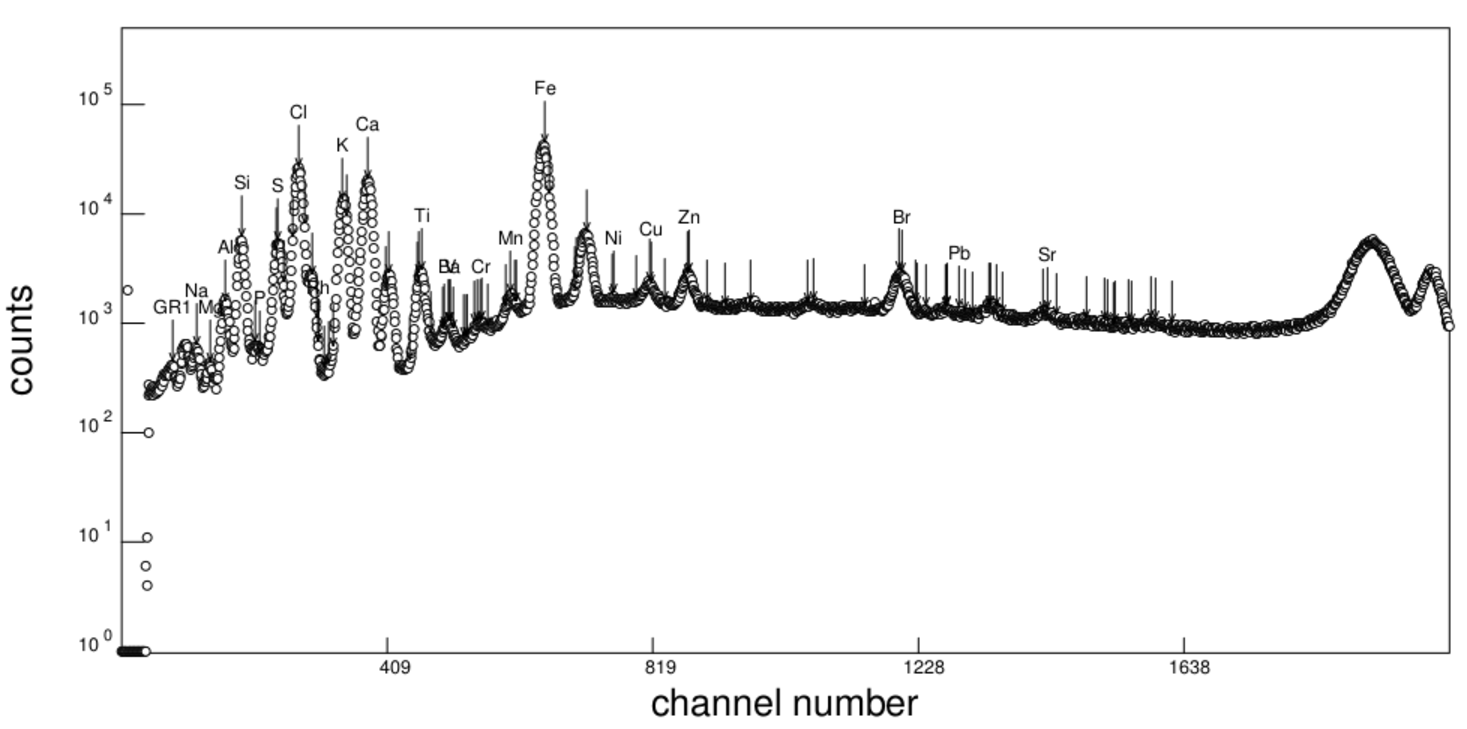
\includegraphics[width=\textwidth]{../inputs/images/winqxas/GHA41editado.pdf}
    \caption{Espectro de amostra carregada (GHA41) - Acra Nima}
  \end{subfigure}
  \begin{subfigure}[b]{0.7\textwidth}
    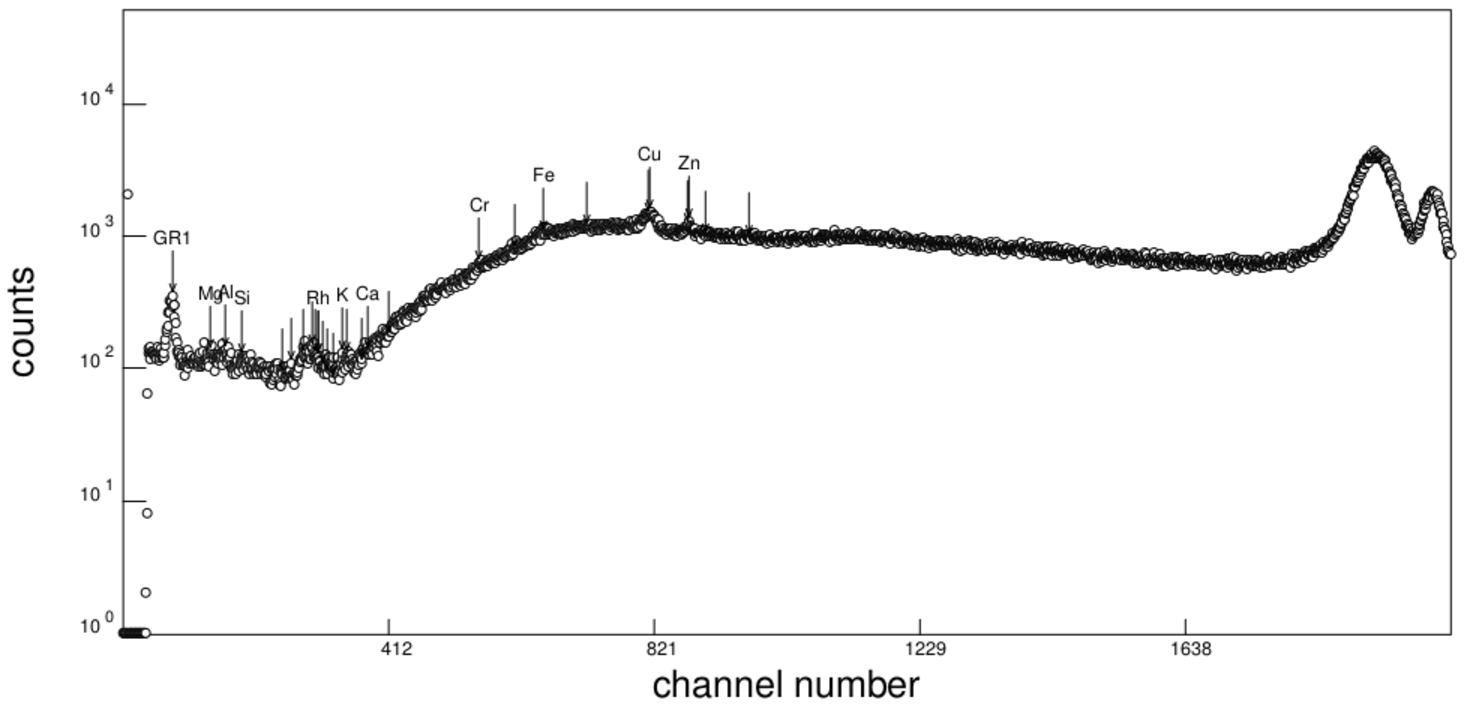
\includegraphics[width=\textwidth]{../inputs/images/winqxas/GPE770editado.pdf}
     \caption{Espectro de amostra branca (GPE770)- Acra Nima}
  \end{subfigure}
  \caption{Espectros amostra branca e carregada \label{fig:winqxas}}
\end{figure}

Na análise feita nos espectros, pico a pico, deve-se ter atenção 
para identificação e correção dos seguintes eventos quando há picos com 
muitas contagens: 

\begin{itemize}
  \begin{spacing}{1.0}
  \item pico soma: quando fotóns do diferente elementos são contados
        juntos pelo detector. 
  \item pico escape: quando o fóton incidente excita o silício do detector
        e é contato com a energia menor, pois parte foi usada na excitação 
        do silício. 
  \end{spacing}
\end{itemize}

A seguir, apresenta-se a calibração do multicanal, ajuste linear entre canal 
e energia encontrado a partir de pelo menos dois elemento conhecidos do 
espectros:

\begin{equation}
  E = 0,0101 \cdot Canal - 0,1335 (keV)
\end{equation}

%%%%
\subsection{Limite de detecção}

O limite de detecção (LD) é a intensidade mínima do pico de um elemento para haver 
detecção da espécie considerando-se o tipo de filtro e XRF-ED empregados. 
Irradiando-se uma amostra branca obtém-se o número de contagens 
medidas ($N_{fundo}$) sob o pico (fundo do espectro) de cada um dos elementos
medidos.
As contagens de fundo do espectro seguem uma distribuição de Poisson e portanto 
a incerteza para o valor de N contagens é $\sqrt{N}$.
Desta forma, adota-se como LD para um elemento, que as contagens de seu pico 
característico seja pelo menos três vezes a incerteza na contagem de fundo:

\begin{equation}
  \label{eq:limitedeteccao}
  N_{LD} = 3 \sqrt{N_{fundo}}
\end{equation}

Pode-se calcular o LD em termos da massa elementar com a 
equação \ref{eq:xrfedmassa}. O limite de detecção muda conforme a quantidade de 
material coletado, sendo maior em amostras carregadas, devido à sobreposição de 
picos e a maior reflexão do feixe na amostra.

Assim, o ideal é calcular o LD em cada amostra, mas ele deve situar-se entre 
aquele medido em um filtro branco e uma amostra com bastante carga.
Os LDs encontrados para os dois tipos de amostras estão apresentados 
nos gráficos da figura \ref{table:ld} em termos de concentrações típicas 
($\mu g / m^3$) para o volume médio de 13,9 $m^3$. 
Note-sa que na linha K o LD é alto para elementos de baixo número atômico, 
dificultando a detecção desses elementos, mas melhora com o aumento de Z. 

\begin{figure}[H]
  \begin{subfigure}[b]{0.5\textwidth}
    \includegraphics[width=\textwidth]{../outputs/limitDetectionK.pdf}
    \caption{linha K}
  \end{subfigure}%
  \begin{subfigure}[b]{0.5\textwidth}
    \includegraphics[width=\textwidth]{../outputs/limitDetectionL.pdf}
    \caption{linha L}
  \end{subfigure}
  \caption{Limite de detecção em termos de concentrações típicas 
           ($\mu g / m^3$) para amostra branca e carregada.
           \label{table:ld}}
\end{figure}

\begin{table}[H]
  \centering
  \input{../outputs/LD.tex}
  \caption{Limite de detecção para XRF-ED calculado com amostra branca e
           carregada. \label{table:LD}}
\end{table}
